\documentclass[12pt]{extarticle}
\usepackage[utf8]{inputenc}
\usepackage{cite}
\usepackage{graphicx}
\usepackage[margin=1in]{geometry}
\usepackage[square,sort]{natbib}


\title{Variational Auto Encoders \\  \large A deep learning approach to dimensionality reduction \\and generative modelling}
\author{Una Singo \\ Marcus Gawronsky }
\date{September 2019}

\begin{document}

\maketitle


\begin{abstract}
Variational Autoencoders (VAEs) are a class of generative artificial neural network commonly used for dimensionality reduction in machine learning applications.  In this paper, we implement a stable Variational Autoencoder and benchmark its performance against traditional methods in multivariate statistics using common open data sets. We build on our implementation with two experiments; the first is an application to noncolumnar data in the medical field, and the second is an original generative sampling problem.   
\end{abstract}



% \newpage
% \section*{Introduction}

% A Variational Auto Encoder (VAE) is a type of neural network that allows for efficient dimensionality reduction on large datasets by computing some non-linear projection into a latent space. These latent feature spaces are assumed to have distributional properties that allow for generative sampling and so the network is trained to learn the set of encoding and decoding parameters that will generate samples that simulate the distribution of the input dataset \cite{vaeBayes}.  \newline
% A VAE manages to pose dimensional reduction as a supervised learning problem, in which a neural network is trained using two weighted loss functions to reconstruction its input from a lower dimensional latent space.  These two loss functions can vary based on the given domain or data but feature a reconstruction loss, commonly the chosen to be the mean-squared error or cross-entropy between the output and the input, and penalty on the distributional properties of the latent space, commonly the Kullback–Leibler divergence. 
% \newline 

% \begin{figure}[htp]
%     \centering
%     \includegraphics[width=8cm]{encoderdecoder.png}
%     \caption{Diagram of how the data flows through the VAE}
%     \label{fig:diag}
% \end{figure}
% Figure 1 aims to show the VAE architecture. The data $\mathbf{X}$ is assumed to be an $i.i.d.$ high dimensional dataset and the latent variables are denoted as $\mathbf{z}$ are assumed to follow an unobservable distribution. The encoder network is defined as the conditional probability distribution $q_{\theta}(\mathbf{z}|\mathbf{x})$ and outputs estimates to $q_{\theta}(\mathbf{z}|\mathbf{x})$ which is assumed to follow a parametric probability distribution. Using the estimated parameters from the encoder neural network, sample values of $\mathbf{z}$ are computed and used as an input to the decoder neural network $p_{\theta}(\mathbf{x}|\mathbf{z})$ which outputs estimates to the conditional distribution $p_{\theta}(\mathbf{x}|\mathbf{z})$ which can be used to sample values of $x$. \newline


% In recent years the theory of VAEs has been extended on significantly in work by \cite{zhao2017infovae} and \cite{tolstikhin2017wasserstein} to apply other loss functions on the distribution of latent space with much success. Additionally, the flexibility of the VAE has found application in computer vision, natural language and time-series modelling with the use of Recurrent and Convolutional Neural Networks as encoder and decoder networks to compress, de-noise and generate new images or time-series. The VAE has also been developed alongside Adversarial Methods such as Generative Adversarial Networks to produce Adversarial Autoencoder which provide state-of-the-art performance on tasks such as image synthesis.  

% \subsection*{Objectives}
% Our aim is to produce a stable implementation of a Variational Autoencoder which we may compare against a common benchmark dataset found in the deep learning literature. Using this model we will investigate the strength of this method when compared to similar such techniques in dimensionality reduction.  We aim to build upon our implementation to explore the application of this methodology to various domains such as computer vision and aim to then explore the application of this method to a public dataset related to a specific field of research.  

\newpage
\section*{Literature Review}
Variational Autoencoders (VAEs) are a class of generative artificial neural network commonly used for dimensionality reduction in machine learning applications.  The technique extends on the application of traditional autoencoders and deep belief networks by introducing techniques from Variational Bayesian Methods.  \\
\newline
An autoencoder consists of two neural networks, an encoder network and decoder network. The encoder network takes an input and produces a lower-dimensional representation of the data. The decoder network takes the lower-dimensional representation of the data and learns a reconstruction of the data back into its original vector-space. These neural networks can have a varying number of hidden-layers, activation functions and neurons to learn non-linear representations of the data \citep{Bengio2007, Bengio2013}.\\ \newline
Variational Bayesian Methods are a class of techniques used in approximating intractable integrals found in Bayesian Modeling.  Using an approximate distribution, $q^\star(x)$, a loss function is used to minimize the difference between the approximate distribution and true posterior.  This loss function is often chosen to be the Evidence Lower Bound (ELBO) or Kullback–Leibler divergence and is weighted in the optimization procedure to ensure the validity of the applied approximate distribution.   
\newline
The Variational Autoencoder aims to extend on encoder-decoder model architectures by placing distributional assumptions on the low-dimensional latent space.  By making this assumption, these models can be generative, allowing one to sample data across a complex data manifold.  While several methods can be used to ensure distributional assumption, the original authors include the Kullback–Leibler divergence into the loss function of the model to ensure a distribution over latent variable which is approximately standard normal \citep{vaeBayes, zhao2017infovae, tolstikhin2017wasserstein}.  
\\

\noindent Using these techniques, Variational Autoencoders provide a flexible method which can be applied to solve a wide range of problems across domains. In the original paper,  \cite{vaeBayes} use the popular MNIST dataset to both embed and generate new images of handwritten digits. A significant number of subsequent research on VAEs has focused on the learning latent distributions of images and generating new images. Generative Adversarial Networks are a popular example of such research outputs where the objective is to generate fake images that appear to be authentic to human observers \citep{Goodfellow2014}.  \newline 
Apart from image generation VAEs have been shown to solve anomaly detection problems. \cite{An2015} propose a method using the reconstruction probability from a variational autoencoder to identify outliers. Their experimental results show that this method outperforms traditional auto-encoder and principal components based methods.



\newpage
\bibliographystyle{apalike}
\bibliography{M335}

\section*{Appendix}
\begin{figure}[htp]
     \centering
     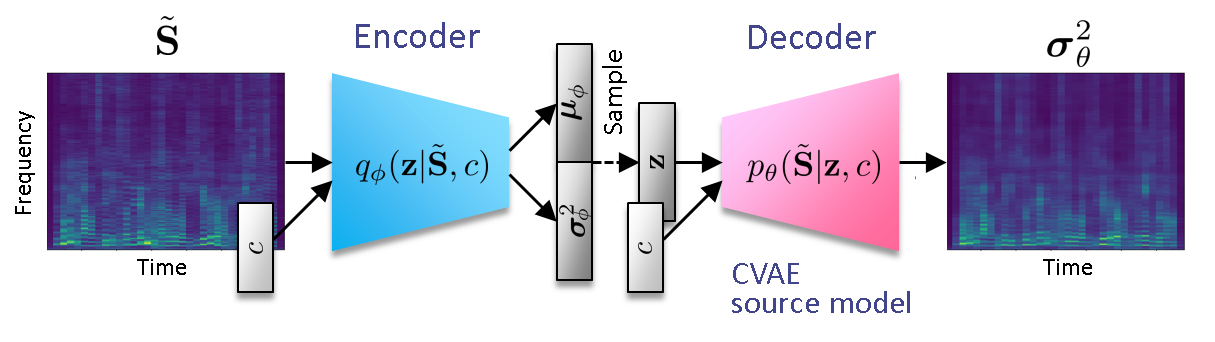
\includegraphics[width=15cm]{VAE.png}
     \caption{Diagram of how the data flows through the VAE \cite{Kameoka2019}}
     \label{fig:diag}
\end{figure}

\end{document}
